\lhead{\emph{Design}}
\chapter{Design}
\label{sec:design}
In this chapter the design of the system is described. Although we have decided from the beginning to design a system based on head gestures and audio modalities, we will still discuss how alternative modalities based on existing systems and related research from chapter \ref{sec:relatedwork} would fit in a biking scenario. This will give a better insight of the importance of modality choice - the benefits and tradeoffs - when designing systems for interaction in-motion. Also the related systems could contribute to the design of specific features for our final system. This is part of the design rationale and covers the first part of this chapter. In the second part the final system design is presented.


\section{Design Rationale}
% Intro
Before choosing a design for a system different factors needs to be considered e.g. the reasons behind design decisions and the justification for it; other design alternatives considerations and the tradeoffs when choosing a design over another; the argumentation that lead to the design.

% Ubicomp challenges
When designing for ubicomp new aspects needs to be taken into consideration which increase the complexity of the system e.g. different devices, mobile users and changing environment and context \cite{barfield_fundamentals_2000}. Also we note that we are not only designing user interfaces but also the interactions between a user and the system through artifacts embedded in the environment \cite{beaudouin-lafon_designing_2004}. Furthermore it should be taken into account whether the interaction happens while the user is in motion as this introduces even more complexity as decribed earlier in section \ref{sec:interactioninmotion}.

In this project we have defined the following requirements of the system: A user should navigate a music player, or more precisely explore and select music tracks, while biking. In other words we have a user interacting with artifacts while biking in a traffic environment, implying user awareness of road conditions, cars, other bikers, etc.

As a consequence of these requirements, we will in the next sections discuss the constraints emitting from a scenario like that and how modality combinations could fit in the design of such a system. This will result in a discussion on related systems, that uses the audio modality as interaction form. Last we will delve further into specific related audio interfaces and look at different auditory menu designs.

\subsection{Biking scenario constraints}
% intro, physical and mental constraints
Several constraints emerge from a humans capabilities to interact with a system while biking, both physically and mentally. Seen from a physical perspective the person riding the bike needs to have both hands on the handlebars in order to dodge any sudden obstructions e.g. an inattentive car. For the same reasons, and more importantly, the persons eyes needs to focus on the road. The latter is of more importance from the fact that people can not easily divide their visual attention between tasks \cite{brewster_overcoming_2002} but two hands can work independently from each other, dedicating one for steering and one for the interface. This does not mean that one hand can steer a bike perfectly - this is subjective, and we must assume that both hands for steering is preferable. Lastly biking requires the legs/feed on the pedals to move forward. From a mental perspective biking is heavily depending on the users attention or perceptual load first of all to navigate the road but more importantly to keep the ability to react to traffical events. This perceptual load is complemented by the cognitive load which can increase in a very busy traffical biking scenarios and depends on the users ability to handle such scenarios.

From a system perspective a biking scenario also implies constraints. First of all interaction with the system should preferably go through some kind of wearable device or at least something easy installable hardware that could be attached to the bike. The system also needs to optimize handling of unintentional interaction during biking e.g. motion gestures when riding a bumpy road. Secondly and most important the system needs to aim for minimizing the workload required by the user - every added feature should be considered i.e. every interaction task should be considering conducted while biking. Also the content presented to the user should be considered in terms of the interaction modality being used e.g. in a visual music player interface artist/track information and a lot of navigation possibilities might be good but if the same information and functionality were to provided via audio this would cause a non-linear effect and add too much complexity to the system.

\subsection{Modalities reasoning}

% HMD, Gaze tracking
\textbf{Visual challenges}

A headmounted visual display like Google Glass would give total hands-freeness when biking but as mentioned in \ref{sec:interactioninmotion} such displays can be hard and obtrusive to use in bright daylight. Also such interface still would require the visual attention from the user \cite{geelhoed_safety_2000}, although the user would not have to change head direction while biking (like when looking down on a traditional stop-to-interact interface). Same arguments follows with a gaze tracking solution. Also such a solution could require some kind of installation on the bike e.g. a camera attached to the handlebars for tracking the eye. Mobile solutions exists \cite{mardanbegi_eye-based_2012} but this will still imply the user to look at the device, and probably hold the device i.e. occupying one hand, while interacting. However the benefit with using visual displays like the headmounted displays in our scenario is, that it's possible to keep the rich visual experience of exploring music tracks before selecting them - information could be linearly translated from the stop-to-interact music player interfaces. It can be argued though, that the experience is not as rich when biking in a traffic environment where attention is divided.

Studies on multimodal interaction \cite{zhao_shared_2013} have shown that when humans needs to attend a physical visual task and a virtual task at the same time (dual task situation) - they found it significantly distractive to attend to the virtual task in a visual way. Instead audio has shown to be less distractive. The biking while interacting scenario can easily be translated into such a dual task where the physical task is to attend to the road and traffic and virtual task is to explore and select music tracks. Inspired from this and from other studies showing that audio can improve usability with mobile devices in eyes-free mobile conditions \cite{brewster_multimodaleyes-freeinteraction_2003}, systems designs that uses audio modalities should be considered instead.

% Audio interfaces/related systems
\textbf{Audio modality combinations}

% voice recognition
Using audio both as input and output modality would imply some kind of voice recognition system like the Google Search voice command system for Android mentioned in section \ref{sec:alternativemusicuis}. A good thing about this system is that the hardware requirements are minimal - it would work on all devices supporting Android and with all kinds of headsets. From a physical and workload demanding perspective this could work in a biking scenario e.g. a user would have to pick out the phone (maybe from the pocket) and then place it near the mouth and give the command. The visual attention would still be on the traffical surroundings although picking out the phone could need some attention. By using a headset controller with a mic this possible "hand attention problem" could be avoided. This interface however have some challenges \cite{sawhney_nomadic_2000} especially in noisy environments, where voice commands can be hard to recognize by the system, making it tedious and frustrating for the user to keep repeating the command. This frustration and also that the user is doing a physical activity like biking (increasing heart rate), can change the voice and affect the systems recognition abilities. At the same time these commands are limited i.e. navigation is limited. Too many commands would add heavy complexity to the system e.g. imagine a stop-to-interact music player interface like Spotify to translate just 10 of their navigation features to a voice command system. This will create a non-linear effect i.e. the user will have a hard time just remembering the commands and could get lost quickly in the navigation.

% touch based
Touch and audio based interfaces also suffers from limited navigation controls. Todays headset music controllers however fits well in a biking scenario. Although using one hand while biking to navigate the interface, the time it takes to push a button is short i.e. reducing the time where the bike is controlled with one hand. This short navigation maneuver is also due to the limited possible interface controls. Similar to these head controllers are the touch based interfaces that uses touch screens \cite{pielot_pocketmenu:_2012, pirhonen_gestural_2002} - controlled from the pocket. These interfaces however uses more advanced output modalities e.g. audio/tactile simultanous modalities (PocketMenu) and spatial audio feedback, which potentially could be used for richer exploration of menu items but also possibly increase complexity i.e. making it a harder cognitive task. Considering these advanced output modalities spatial audio has shown to be able to present complex information \cite{bronkhorst_cocktail_2000, gaver_sonicfinder:_1989} while keeping the human cognitive load down \cite{vazquez-alvarez_eyes-free_2011} and in combination with gesture input modalities, it was used effectively when navigating an interface in eyes-free mobile conditions. 

Considering combining spatial audio output with a motion gesture input modality, possible available human body parts when biking could be hands (implies biking with one hand) or the head. Although feet as a modality input were evaluated in a running scenario with good results \cite{smus_running_2010}, it would be awkward when biking would require both feet on the pedals to keep moving. Kajastilas free-hand gestures \cite{kajastila_interaction_2013} would imply the same hand interaction challenges discussed above but also a camera installed on the bike to detect the movements. Sensors could be used instead but would require some artefact installed on the hand. Instead it would be more appropriate to install sensors into a headset and use head movements as input modality like \cite{park_gaze-directed_2011, brewster_multimodaleyes-freeinteraction_2003} as this would not add any additional artefacts to the system. When using head gestures it would still be possible to keep the eyes on the road, assuming the head rotation is not too big. Also the human head itself is physically constrained in that it can be rotated 140 degress for shaking and 100 degrees for nodding \cite{lopresti_neck_2000} which should be taken into consideration when designing the auditory menu. Also when biking motion gesture detections could be unintentionally activated e.g. an accelerometer sensor value increases when moving forward.

With the chosen modalities of head gestures and spatial audio we will next compaire auditory menu designs that uses these modalities and discuss their customizability in a music listening biking scenario.

\subsection{Auditory menus}
To achieve the first goal of this thesis that is, to design a mobile music player interface based on head gestures and 3D audio that allows a user to explore and select music tracks, we have discussed the interaction scenario constraints above and the suitability of modality choices, but we also need to consider the minimum requirements of the system: The exploration and selection of music tracks. This is more related to the content of the system and how it is presented. To compete with existing "stop-to-interact" music player interfaces in terms of this, we need to translate as much of the visual information into audio feedback without causing any non-linear effects.

One advantage with using a multimodality combination of head gestures and spatial audio is that it can provide natural interaction \cite{gaver_auditory_1986} i.e. hearing sounds as we would normally do in the real world in relation to head direction. Another advantage with spatial audio is that it can enable the "cocktail party effect" \cite{bronkhorst_cocktail_2000} i.e. people can segregate multiple simultanous playing sounds. Imagining if exploring simultanous playing music tracks is feasible, that could provide a rich exploration factor to our music player interface - allowing the user to hear tracks before selecting them.

Although Park et. al \cite{park_gaze-directed_2011} showed good results with a 2D grid menu it is hard to localize vertically positioned sounds compaired if they were aligned horizontally - especially if they play simultanously. A circular egocentric menu layout showed the best evaluation results in the head gesture system by Brewster et. al \cite{brewster_multimodaleyes-freeinteraction_2003} but they were limited to 4 sound items because of head movement constraints (a nod in 45 degrees is hard for a human to conduct). Although same study showed that an exocentric layout were slower it would give a more natural selection (directing the head against an item and selecting it) and provide the opportunity for more than 4 sound items.


\section{Spatial Music Menu}
This section contains a description of the system design. The physical design of the system assumes artefacts in form of a headset, which can detect head gestures by using built-in motion sensors and deliver 3D audio feedback, that communicates with a mobile device put in the users pocket during biking.

\begin{figure}[t]
	\centering
		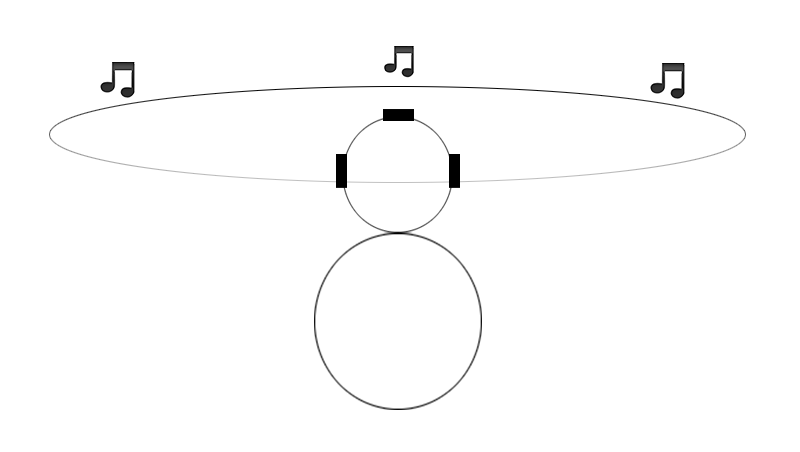
\includegraphics[width=0.6\textwidth,height=\textheight,keepaspectratio]{./Figures/sounddesign.png}
		\rule{35em}{0.5pt}
	\caption[Soundscape Design]{Soundscape Design - Visualising how the circular auditory menu surrounds a person (viewed from the persons back)}
	\label{fig:sounddesign}
\end{figure}

\subsection{Soundscape design}
Non-speech sound items (music tracks) are layed out in a horizontal circular way within 140 degrees in front of the user, see figure \ref{fig:sounddesign}. The number of music tracks are spatially positioned and are playing simultanously. The menu uses exocentric interaction - by turning the head towards a music track, it will move in the center of the users front audio space. We conducted a small pilot study where 2 kinds of design were tested. The two designs can best be described by imagining a carousel turning, while different koncerts play around it. In the first design the user stands in the center of the carousel looking out and in the second the user stands on the edge of the carousel looking out. These two interaction modes are illustrated in figure \ref{fig:interactionmodes}.

\begin{figure}[t]
	\centering
		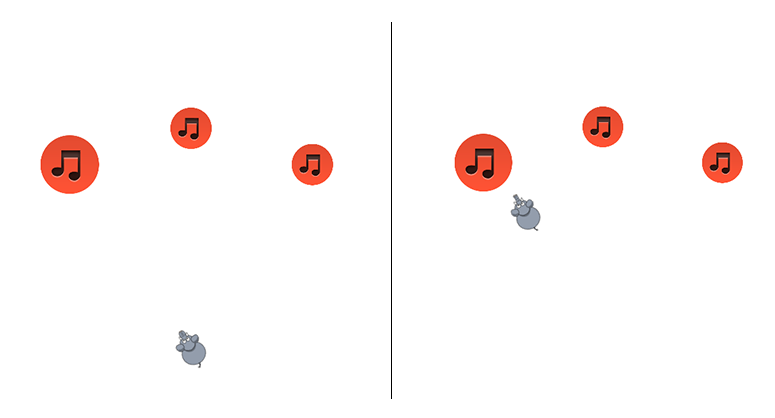
\includegraphics[width=0.9\textwidth,height=\textheight,keepaspectratio]{./Figures/interactionmodes.png}
		\rule{35em}{0.5pt}
	\caption[Interaction modes]{The system consists of two different interaction modes - with (to the right) and without (to the left) zoom feature. The user is illustrated by an elephant looking at the sound items.}
	\label{fig:interactionmodes}
\end{figure}

The purpose of the pilot study was to give qualitative feedback and specify appropriate parameters like max number of simultanous playing music tracks, the preferred degree for head rotation and the distance between the user and the music items. Although not neccesary for the final design, we developed a hifi-prototype \cite{benyon_designing_2010} that visualised the actual soundscape design. This envisionment technique gave the users in the pilot study a quicker and better understanding of the design. Figure \ref{fig:pilotstudy} shows a user testing the design and the hifi-prototype.

\begin{figure}[b]
	\centering
		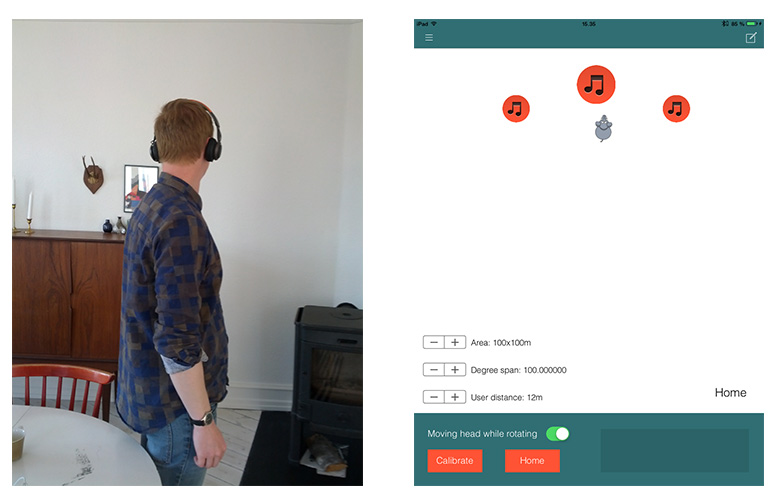
\includegraphics[width=0.9\textwidth,height=\textheight,keepaspectratio]{./Figures/pilotstudy.jpg}
		\rule{35em}{0.5pt}
	\caption[Pilot study]{Pilot study showing a user testing the design and the visual prototype.}
	\label{fig:pilotstudy}
\end{figure}

The pilot study consisted of 5 participants, 4 males and 1 female. The music tracks used in the test were added by the users to make sure they knew the tracks. The experiment were conducted by observation and semi-structured interviewing \cite{benyon_designing_2010}. Both interaction modes were tested by starting laying out 3 sound items and then adding 1 until the user found it to hard to recognize the music tracks. Distance and head rotation parameters were adjusted to match the user preferences every time sound items were added. The users preferred the interaction mode with zoom effect and they felt comfortable with 6-8 simultanous playing music tracks compaired to the other mode where \textgreater 4 simultanous music tracks were hard to segregate. Users preferred a smaller head rotation degree with the zoom effect of 80-100 degrees compaired to the other mode where 120-140 degrees were preferred. The feedback results are shown in table \ref{tab:pilotresults}.

\begin{table}[t] 
\scriptsize
\centering
\caption{Pilot study feedback} % title name of the table 
%\centering % centering table
\begin{tabular}{L{3cm}C{3cm}C{3cm}} \toprule
	 & Direction based & Direction based with zoom effect \\ \midrule
    Max number of music tracks   & 3-5 & 6-8 \\
    \\
    Preferred head rotation degree   & 120-140 & 80-100 \\ \bottomrule
\end{tabular}

\label{tab:pilotresults} 
\end{table}

\subsection{Navigation}
The menu was designed with a 2 level exploring part that utilizes the soundscape design and a final level for playing the music track (simple playback). The idea is that the exploring starts by selecting an artist (HOME), then moving down a level to select a track from that artist (ALBUM) and then finally playing it (PLAYING TRACK). This menu hierachy (reversed) is illustrated in figure \ref{fig:navigation}.

\begin{figure}[b]
	\centering
		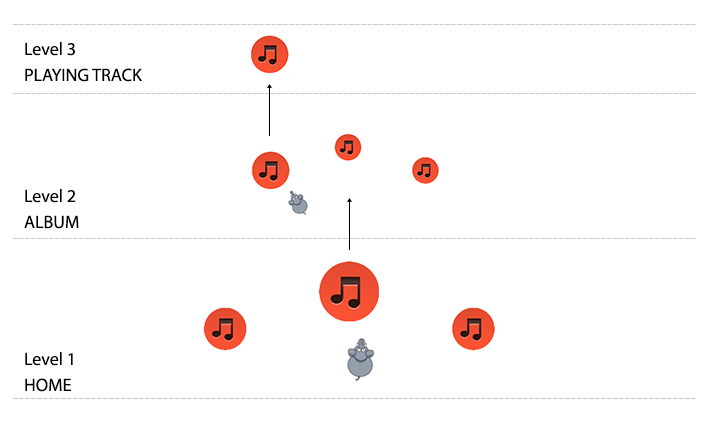
\includegraphics[width=0.8\textwidth,height=\textheight,keepaspectratio]{./Figures/navigation.png}
		\rule{35em}{0.5pt}
	\caption[Menu Hierachy]{The menu consists of 2 exploring levels and 1 level for playing track.}
	\label{fig:navigation}
\end{figure}

To navigate between levels simple head gestures were designed: A forward nod for going up one level, a backward nod for going back one level and a right sideways nod for activating the menu. Activating the menu would the case where a music track is playing and the user wish to change track - it will take the user to the HOME level. When entering a level, audio feedback is given in form of speech recorded sounds telling what level the user is in e.g. "Home", "Album" and "Playing track". These head gestures and the ability to navigate between menu levels were evaluated in a second part of the pilot study mentioned above. Participants started by recording the three gestures to get some training data. Then the participants simply tried to choose tracks by navigating between levels using the gestures. The system seemed to react to undesired gestures (true negatives) when participants were rotating the head which affected the navigation experience. Backward and sideways nods were removed and instead to go up one level or to activate the menu a simple push on a button on the headset were introduced. This helped in several ways - the user only needed to focus on 1 gesture which they also reported was the easiest one to conduct. For the systems point of view the nod is the most important gesture in that it is the actual selection of an item. We assume users to most of the time select the desired music track, and therefore going back a level would at least not be as neccesary as selecting i.e. we would not expect a lot of button push activity. Same theory goes for activating, this will be a 1 time push for every time the user wishes to change track. An accuracy test were conducted for nod selections by observing the user and the system response registering true postitives, true negatives and false positives, see table ??

TODO: table and short resume of accuracy results




















% OLD - Use some parts here and move some to introduction method section


%The design is based on the following parameters: 

%\begin{itemize}
%\item Simultanous sounds (music tracks) spatially positioned
%\item Horizontal circular menu layout with music tracks as menu items
%\item Non-speech sound items in form of music tracks
%\item Simple speech sound feedback indicating menu level
%\end{itemize}

%- Music, strength of recognizing artist/track through listening vs seeing the text on a screen
%- Horizontal argument
%- Two menu interaction modes, distance/
%- Selective attention task
%- Simultanous sounds, exploring, cocktail party effect argument
%- Experimental design, sounds perceived, zoom effect, user should detect sound direction (which track)

% Horiontal alignment

% Circular

% non-speech sound

% selective-attention

% exocentric

% Head gestures, nod=yes




\begin{comment}

This chapter first explains the design methods used and the most important design activities and choices made in the design process. Based on this process the final prototype design is presented at the end of the chapter.

\section{Design model and methods}
In this section the model used for designing the final prototype is presented including the different techniques used throughout the design process.

The related works conducts the foundations for an early first prototype. This prototype will then go through an iterative design process, taking a user centered approach. This will enable specifications to emerge during the process and these learnings and modifications will result in new experiments and prototypes. This iterative design model is illustrated in figure \ref{fig:iterative}.

\begin{figure}[t]
	\centering
		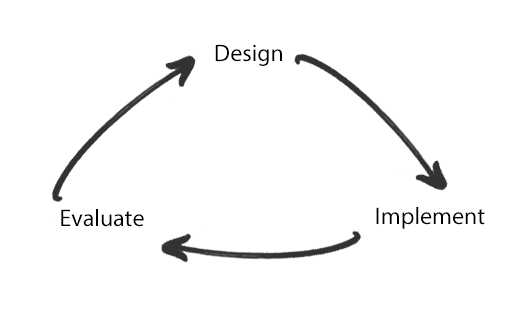
\includegraphics[width=0.6\textwidth,height=\textheight,keepaspectratio]{./Figures/iterative.png}
		\rule{35em}{0.5pt}
	\caption[Iterative Design Model]{Iterative Design Model}
	\label{fig:iterative}
\end{figure}

\subsection{Envisionment}
One of the goals with the final system is that it should be eyes-free i.e. the user should not depend on a visual screen UI at the end. Despite this goal, the use of a screen to visualize e.g. a virtual menu, can be helpful in the design process. This will enable test users to get a quicker and better understanding of how the interaction works. In this design process a mobile device screen will be used for envisionment - this is also called a hifi prototype or software prototype \cite{benyon_designing_2010}.

More concretely audio sources and the users head position including rotation will be mapped visually to a screen dynamically during user interaction. An example of this screen is shown in figure ?

\section{Design process}
This section starts out by describing the first experimental prototype design inspired from previous research work and then each iteration including user feedback and design changes and experiments. More specifically the design completed 2 iterations before the final prototype design.

\subsection{Initial prototype design considerations}
Before we started to reason about initial design choices we started out by defining what the system actually needed in order to evaluate and revise the hypothesis from the problem statement.

% intro, track exploring
First of all we wanted the system to be able to play music. This is in itself a trivial task but as we the same time wanted to control the system only with with head gestures and audio output a traditional music player includes too many options e.g. play, pause, stop, next/previous, volume, equalizer, track exploring, etc for the scope of this thesis. All the alternative music players mentioned in chapter \ref{sec:relatedwork} is limited to simple commands like play, stop, next/previous and volume. Taking it a step further we wanted to evaluate the track exploring part i.e. navigating to a preferred track and playing it. This made et clear that some kind of auditory menu with tracks as menu items was needed and although not music players the related systems from chapter \ref{sec:relatedwork} using auditory menus could inspire to an intital menu design.

% Auditory menu, exocentric, head rotation constraints
When looking at the different related auditory menu designs we needed to find a design that fitted into the context of the user activity i.e. biking and also user interaction modality. E.g. in a biking scenario the user should have eyes on the road thereby constraining the head rotation. Park et. al \cite{park_gaze-directed_2011} showed good results with a 2D grid menu. It should be taken into account that their audio output consists of simple speech commands e.g. speech recorded numbers. We want to present multiple music streams (non-speech audio) and studies have shown that when presenting multiple non-speech audio streams simultanously in a spatial audio space, segregating the audio streams horizontically has a better effect than vertical alignment [TODO: ref]. It seemed that a circular auditory menu could be a good starting point and both Kajastila and Lokki \cite{kajastila_interaction_2013} and also Brewster et. al \cite{brewster_multimodaleyes-freeinteraction_2003} evaluated this kind of menu design with good results.

[TODO: Image/prototype sketch?]

% Circular menu design, head gestures
While placing music streams in a circular way around a users audio space we needed a way of navigating to and chosing a specific track. The Brewster et. al \cite{brewster_multimodaleyes-freeinteraction_2003} system uses directed nods to choose an item but this limits the number of items to 4 (1 for every 90 degrees) as a nod in 45 degrees

The inititial interaction design was inspired from Kajastila and Lokkis system although they used hand gestures as modality input. 

For navigating and choosing menu items

[TODO: egocentric vs exocentric audio output, Brewster system good ref \cite{vazquez-alvarez_eyes-free_2011}]

% Summarising

[TODO]
In this project multiple audio sources (music tracks) are presented for the user at the same time but none of them requires a respond i.e. the focus is on selective-attention tasks.

\end{comment}





% OLD


% From wiki:
% - the reasons behind a design decision,
% - the justification for it,
% - the other alternatives considered,
% - the trade offs evaluated, and
% - the argumentation that led to the decision.









